\documentclass{standalone}
\usepackage{tikz}
\usepackage{ctex,mhchem}
\setCJKmainfont{Noto Serif CJK SC}
\usepackage{mhchem,siunitx}
\begin{document}
\small
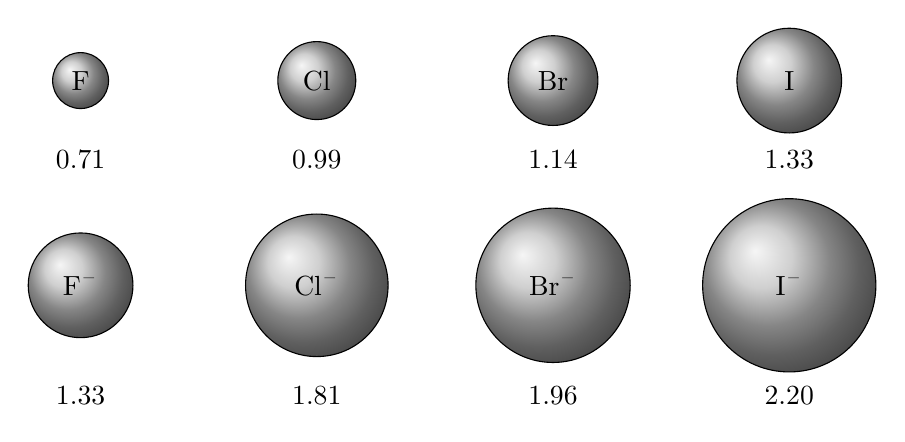
\begin{tikzpicture}[>=stealth]
  \foreach \x/\r/\R/\a in {0/0.71/1.33/F,3/0.99/1.81/Cl,6/1.14/1.96/Br,9/1.33/2.20/I}
  {
    \draw[ball color= lightgray] (\x,1)circle(0.5*\r)node{\ce{\a}};
    \node at (\x,0){$\r$};
    \draw[ball color= lightgray] (\x,-1.6)circle(0.5*\R)node{\ce{{\a}-}};
    \node at (\x,-3){$\R$};
  }
\end{tikzpicture}
\end{document}